\section{Techniques Implemented} 
\label{sec:exp}

After explaining the theory of several approaches we will now describe our implementations. The proposed algorithms are not always fitting to 
the principle of the games or have a lot of parameters that have to be adjusted in order to have good results. We will first point out some basic strategies
such as staying alive.


\subsection{Stay Alive} 

We implemented two different Stay Alive Agents that only have the aim of acting save and are hoped to randomly win the game.
Even if there is the possibility to simulate an action, there is a permanent uncertainty. All objects of the games in our competition
can - but do not have to - act randomly. If we are using the \textit{advance} function that allows us to simulate one step, the result is just one possible state of the future. This implies that even if we are not dying in our simulation we could still die in the real game.

One approach is to simulate the next action $n$ times. If the agent does not die during this simulations, the next action should be safe.
The challenge is to set a good value for $n$. If the value is to large, not all the possible actions can be tested. If it is to small, the probability that the action is unsafe grows.
From the resulting set of safe actions, the final action can be randomly chosen.

\begin{figure}
\centering
\begin{minipage}{.5\textwidth}
  \centering
\includegraphics[scale=0.8]{images/safe.pdf}
\caption{Advancing safe actions}
\label{fig:safe}
\end{minipage}%
\begin{minipage}{.5\textwidth}
\centering
\includegraphics[scale=0.8]{images/safe_grid.pdf}
\caption{Grid search for safe actions}
\label{fig:safe_grid}
\end{minipage}
\end{figure}



Assuming that there is a game situation like in~\cref{fig:safe}, the action \textit{RIGHT} is definitely unsafe, a fact that should be clear after an amount of $n$-actions.

Another idea is to analyse the grid around the agent. Each enemy could only move one field at the grid
in one game step, there is a $5x5$ grid that needs to be analyzed. If an enemy at this grid exists, one action might be unsafe. If not, the avatar will not die.


In~\cref{fig:safe_grid} you can see the action that can be excluded without doing any simulation at the game.
The possible next fields (excluding the agent's position if he is not moving) are marked green. The possible positions
of the enemy are red. The action RIGHT by using the grid search is unsafe. 
At first glance it looks faster and better to only look at the grid, but there might be some problems for unknown games:

One problem lies in classifying the game objects at the grid. The grid search is only successful if we can be certain that this object represents an enemy. Otherwise we also classify walls as unsafe.
Furthermore not every enemy can move in all directions but as a agent we would need a special observer to know that.
Staying alive is just a basic strategy which is extended with some other approaches.




\subsection{Heuristic based} 
 
If the action is safe but randomly chosen, the algorithm is only a little bit better than random search.
Therefore a heuristic is used to evaluate one state and get a score. Knowing the game in advance would be a substantial advantage. Whenever this is not the case, the results might turn out completely different.
One heuristic could be very good, for example in a case in which the agent could kill an enemy. However, if in another game
the enemy will kill us, the heuristic will let us commit suicide.

To fix that, we have two different ideas. On the one hand we could implement a dynamic heuristic that is changing over time
and is learning from the environment. On the other hand there could be a third instance called \textit{Explorer} 
that is learning from the environment and creating a knowledge-base. 
To further use this idea in other approaches, we focussed on the following idea.

During the construction time the agent only explores the environment. 
First of all he creates a list including all the interesting targets that exist in the level. He sends pheromones into the grid targeting all of them and simulates until the agent dies. 
For all the simulation there is a global class - the \textit{Simulator} - that automatically makes inferences from the observations.
The knowledge base is the environment class that contains information about blocking, scoring, winning and losing game objects (sprites).
This two classes follows the singleton pattern and can be created by using the factory (cf.~\cref{fig:sim_classes}).
Additional information that can be seen in the figure is the game detection that will be explained later and the field tracker that keeps 
information about all fields at the grid and how often the agent has visited each one.

\begin{figure}
\centering
\includegraphics[scale=0.5]{images/classes.png}
\caption{Class diagram of the simulator and environment structure}
\label{fig:sim_classes}
\end{figure}


When the explorer finds the winning or scoring objects, a heuristic is initialized. We used a heuristic that 
calculates the distance between two targets by using the Manhattan distance. To reach this target we use an A* 
algorithm with three modifications.

Every game step the A* algorithm is executed from scratch even if the target was found in the last iteration.
We use a safety approach for the first action to ensure that the next action we my choose is safe. For that we
use the principle of the stay-alive agent. The A* algorithm has to keep all the states in memory.
This leads to a very fast growing open list with a multitude of states. We introduce a \textit{maxStates} variable. 
Whenever the open list of the A* algorithm is larger than this variable, the list is cut in a half.
For our simulations, we additionally use the simulator as well as the knowledge base. Normally all children of
a state are added to the open list. However, we only add those children to the list of whom we assume we will get a new position. Since we know from the Environment class which objects are blocking, we can use that information
for a smarter iteration.


\subsection{MCTS} 

The theory of \ac{MCTS} is described in \cref{sec:back}. The standard approach was modified to fit our issue. The whole \ac{MCTS} algorithm is computed in the class \textit{MCTSStrategy} which is used by the \textit{MCTSAgent} and the \textit{MCTSHeuristicAgent}.

Our \textbf{tree policy} iterates trough the tree, starting at the root node. When a node is not fully expanded, a randomly chosen child node is generated. We tried out some other ways to choose the children, but random selection worked best. If we reach a fully expanded node the tree policy uses a modified \ac{UCT} formula

\begin{equation}
 	UCT = \frac{Q_c}{V_c + \epsilon \cdot r} + \sqrt{\frac{\ln{(V_n +1)}}{V_c}}
\end{equation} 

to chose the children node, where \textit{n} is the node and \textit{c} the actual children. \textit{Q} is the reward of a node and \textit{V} the number of visits, more precisely the number of times the \textit{tree policy} had chosen this node. The exploitation term is computed by dividing the reward of the child by the number of visits and a random factor to avoid divisions by zero. This term is big for nodes whose reward is high on average.
When the children number of visits are small in comparison to the others, the second term (exploration) will be big. We tried out some other variants and factors, but this solution has produced best results. It is very close to the original \ac{UCT} formula in section \ref{sec:back}.

The \textbf{default policy} tries to figure out how good the given node from the tree policy is. To do that, a simulation with the correspond state observation and random actions needs to be done. It is repeated until the hypothetical level of the simulated node reaches the before defined maximum (maximal depth of the tree). At the beginning, when the tree is small, more simulations are executed. Later, when we have already grown our tree, only a few simulations are executed.

When the simulation is finished, a reward is generated from the last state observation by the delta heuristic which will be described later. The win, loss and score are being considered.
The \textbf{backpropagation} iterates from the node which was expanded by the tree policy to the root, guided by the father references of every node. To every visited node the reward is added and weighted with a before specified value.


The approach of a \textbf{rolling horizon} has been modified and applied to our problem. The goal of this rolling horizon technique is to save computing power. 
When the act method from the \textit{MCTSAgent} or \textit{MCTSHeuristicAgent} is called, a new \textit{MCTSStrategy} (search tree) is constructed or rolling horizon is executed. The new search tree contains only the root node and has to be built up normally; this costs a lot of computing power and time. The rolling horizon does not build a whole new tree, but it uses the information from the previous call of the act method (from the last gametick). 
One subtree of the previous root node will be the new search tree; it is chosen by checking the last action that was executed and takes the corresponding child as the new root node.
After that the levels of the nodes are updated and the tree is built up normally. This saves some computing power and the according tree is larger than the normal one which yields more checked actions and better results.  

We used the \textbf{open loop} approach, and in contrast to the closedloop approach, the state observation is not stored in the actual node. We only store a sequence of actions in every node which leads from the actual state observation (which represents the root node) to the appropriate node. The tree policy does not need the state observation to compute the \ac{UCT} value. 
Before the default policy is able to generate a random path, the state observation of the expanded node has to be generated. All actions in the path of the node are applied to the actual state observation (from the root node) leading a state observation that represents the expanded node. After that, the random path is simulated and the backpropagation updates the reward values.


When no more time is available the \ac{MCTS} algorithm stops and the agent calls the act method from \textit{MCTSStrategy} to choose the action which will be executed given the \ac{MCTS} search tree. The child node from the root which was \textbf{most visited} is taken, some other approaches that take the node with the highest reward tend to produce only poor results. The \textit{MostVisitedNodeComparator} is used to compare the number of visits. When there are more nodes with equal (and highest) number of visits, the heuristic value is used to select a node. With no heuristic given, a random node from the list of the most visited nodes is selected. The depending action is executed by the agent. 


\subsection{Evolutionary algorithm} 

The theory of evolution has to be mapped to the gaming problem. Each candidate of our population is
a list of actions that could be executed. To evaluate the fitness of a candidate we are using the
simulation function that is provided by the game. 
The score

\begin{equation}
s = \sum_{t=0}^n (H(s_t) - H(s_{t-1}))
\end{equation}

is calculated by using the function

\begin{equation}
    H(s_i, s_{i-1}) = 
\begin{dcases}
    10, & \text{if isWinner}  \\
    -10, & \text{if isLooser}  \\
    score(s_i) - score(s_{i-1}), & \text{otherwise.}
\end{dcases}
\end{equation}

that we called delta heuristic function.

We implemented two very naive operations on the pool. The crossover is done by selecting the action of the first or the second individual by 50 \% (cf.~\cref{fig:crossover}).

\begin{figure}[H]
\centering
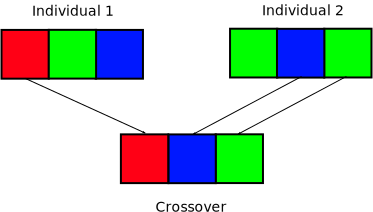
\includegraphics[scale=0.6]{images/crossover.pdf}
\caption{Crossover of an individual}
\label{fig:crossover}
\end{figure}

The mutation is implemented by doing a crossover with a random individual.
For all of our evaluation processes, the mutation probability was set to $0.7$, thus maintaining a crossover probability of $0.3$.

We had several problems with the limited time for the evolution.
For the evolution we want to have a good starting pool and want to reuse our information from the last
game step. All candidates from the last final pool of the last game step have been used for the initialization.


\begin{figure}[H]
\centering
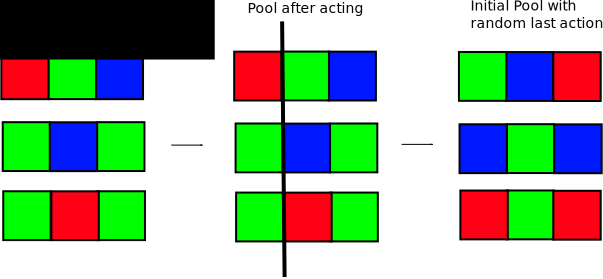
\includegraphics[scale=0.6]{images/sliding_window.pdf}
\caption{Sliding Window}
\label{fig:sliding_window}
\end{figure}

For that we use the principle of a sliding window (cf.~\cref{fig:sliding_window}). The first
action from the last pool is removed because the agent was acting like this at the last game step. To keep the action length fix, one random action is added to the action path.
By using that principle we are not throwing our last simulations away.

Another problem that arises are the differing simulation times for the different games. If we have many game objects that 
need to be updated and checked for collision, the simulation time increases.
However to find a good value for the pool size we need to know the calculation time.
As a fix for this, we introduced the adaptive path length that reduces or increases the actions
of every individual.
For that we must always get the fourth generation. On the one hand, staying at the initial
pool because the evaluation takes to long, will reduce the path length. On the other hand if the agents acts like 
the seventh generation we are bound to have a long period of planning by increasing the path length.

Another problem that we tried to fix is the occurrence of situations where no individual has a positive score or many have a score of zero. This means that no candidate is gaining points. Our first implementations solved such circumstances randomly. 
The randomness could be disabled by using a heuristic. Always using the same heuristic would not work
for all the games because they have different aims. 
This is why we used a heuristic switch after $n$ time steps to have a long time planning strategy.


  
  
\subsection{Game Detection} 
  
Another technique we have implemented is the detection of a known game. We know the 10 games from the test-set and the 10 games from the validation-set; the 10 test-set games are unknown. The Goal of the Gamedetection is to improve the score and the number of wins in the two known game-sets without decreasing the score and the number of wins in the unknown test-set. To do that, the standard parameters of the Algorithm are used when no game is detected; otherwise the optimal parameters for this game are used. These parameters were figured out for some difficult games in which the standard parameters give bad results. To detect a game we generate a String of all Objects (npc, movable, immovable, ect...) and store the Hash value of this String. All the hashes from the known games are stored. In a running Game we generate another String of these Objects and compare the generated hash value to the stored ones. 